%%%%%%%%%%%%%%%%%%%%%%%%%%%%%%%%%%%%%%%%%%%%%%%%%%%%%%%%%%%%%%%%%%%%%%%%
%                                                                      %
%     File: Thesis_Introduction.tex                                    %
%     Tex Master: Thesis.tex                                           %
%                                                                      %
%     Author: Andre C. Marta                                           %
%     Last modified :  2 Jul 2015                                      %
%                                                                      %
%%%%%%%%%%%%%%%%%%%%%%%%%%%%%%%%%%%%%%%%%%%%%%%%%%%%%%%%%%%%%%%%%%%%%%%%

\chapter{Introduction}
\label{chapter:introduction}
\section{Overview}
\label{section:overview}
This chapter gives information about the subject of the thesis, the area of interest with that subject and also general information about current solutions related that topic.

\section{Context}
\label{section:context}

Distributed applications are required in most of central application sectors including e-commerce, e-banking, e-learning, e-health, telecommunication and transportation\citep{thesis:introduction1}. This results that the Internet plays an important role in business, administration and our everyday activities. In distributed applications that share information between each other does not need to be built with same technologies. The fundamental problem is the programming of distributed applications with all the basic interoperability problems involves distributed platforms and heterogeneous components.

On the other hand, Clouds create a new challenge for distribution. They bring new opportunities such as scalability, dynamic instantiation, location independence, application management and multi-tenancy (several users using the same application independently)\citep{thesis:introduction2}. However, they also create distributed platforms and that’s why they need to be able to support distributed applications as easily as possible. That's make importance of interoperability in cloud environment because different cloud providers can have different properties and they need to communicate between each other.

The subject of thesis research current solutions of distributed applications and their implementation in cloud environment and propose the design of the alternative solution that is both simpler and more effective than existing ones.

Taking your Android mobile phone as an example, nowadays a huge part of the people use smartphones that are connected Internet that check news, weathercast or more information like that. Let’s say you have an application in your phone that informs you with current weathercast of your city. That application is most probably written in Java since your phone is using Android system and gets current weathercast over Internet that gets information from weathercast provider, so basically that application asks queries to weathercast provider over Internet and gets response data first and then parse that data and display information to your phone screen. During this data exchange happens, both your mobile phone and weathercast provider must understand each other even they don’t use the same language because the provider could be working in a Cloud provider and written in C\# language. The data is used in C\# and Java is not the same so they will not understand each other naturally. This interoperability (how to interconnect different programs written in different languages, running in different platforms) issue can be solved with current integration technologies such as SOA or REST using XML or JSON over HTTP and both platforms can communicate between each other. Finally you can get last weathercast information from your Android phone or your IPhone using same weathercast provider even they use totally different technologies.

\section{The problem}
\label{section:problem}

Distributed applications need to interact among themselves. In this respect, they need to solve the interoperability problems as any two systems that need to understand each other to achieve meaningful and useful collaboration. The traditional integration technologies, based on either SOA or REST as seen in Figure \ref{fig:soaprest}, is that they use the document concept as the foundation, with a data description language as the representation format and schema sharing as the interoperability mechanism (both sides use the same schema such XML Schema) or using previously known data types. Other factors, such as connectionless protocol (HTTP) and XML, JSON (and by extension SOA and REST) that do not support binary in its main features, because the solutions were also based on text (XML or JSON) and contextual information, are limited for many applications.

\begin{figure}[!htb]
  \centering
  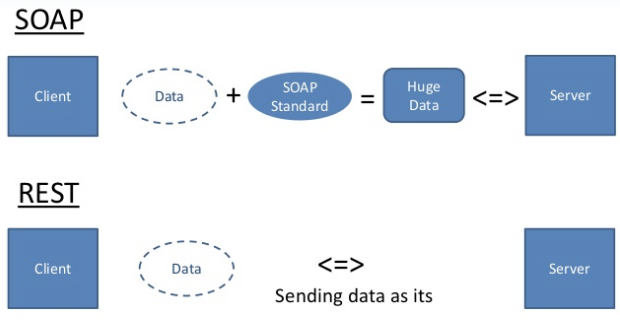
\includegraphics[width=0.9\textwidth]{Figures/soap-rest.png}
  \caption[SOAP and REST Approach.]{SOAP and REST Approach.}
  \label{fig:soaprest}
\end{figure}

The main problem of the traditional integration technologies creates coupling between the provider and the consumer, because both customer and provider are forced to implement full interoperability (for example, sharing a XML schema). This leads to a greater coupling than needed.

While solving data interoperability, the problem of using XML or JSON is that XML or JSON is inefficient in computer terms due to parsing data to build a DOM tree and validating schemas to validate structure of message.

The problem can be explained with an example, as described in the previous example in section \ref{section:context} that you can have two different technologies and they can communicate each other. In case if they use SOA architecture style (namely, SOAP Web Services) you need to use XML (Extensible Markup Language), which both languages can understand easily since, it is a common language. But still you have some steps to deal such as a stub, which is used by a client application to access a remote service. The stub looks like the service interface\citep{thesis:introduction3}; it generates an appropriate XML message and sends it over HTTP then you have XML message that can be read by your mobile phone or weathercast provider and parsed to build a DOM tree to be used. That can be done with sharing same schema to know structure of message. There are some problems with sharing schema which brings coupling problem between systems. So when you want to see weathercast on your phone, firstly your phone creates query message in XML using stub generator then uses HTTP for message transportation. The created message should be validated by schema because if it doesn't obey the schema rules, the provider can not understand the message. When message arrives to provider it validates message regarding the same schema and parses that XML message to own objects to understand it then provide response regarding the query, which is done by your phone application. There are some problems with using XML schema because your phone application or weathercast provider can not alter this schema without informing each other. That creates coupling between mobile application and weathercast provider. After message creation by weathercast provider, this response again needs to be converted to XML message using stub generator and send that response message to your phone. Now, your phone uses XML schema and XML parsers to understand XML message and uses these data to display information to you. As seen in that example it is not very easy to communicate systems that use totally different technologies. In case of REST, you can use different message format instead of XML, for example, JSON which is easier to parse and less heavier than XML, but in REST both languages need to know message structure, then they can parse and understand.

In case of REST, there are some differences. If your weathercast application uses REST to communicate with weathercast provider then you don’t need to create XML message to send weathercast provider. You can use other formats to send it using HTTP to server. Assume that you use JSON and your mobile phone creates query in JSON format then it needs to know unique URl of weather cast provider and HTTP verbs (GET, POST, PUT, and DELETE) because in REST, different HTTP methods can be used with using the same URl. When a message arrived to weathercast provider this message will be parsed with DOM parsers to understand query. In that case your phone and weathercast provider must know structure of JSON message than they can both understand each other. REST may seem more flexible, in the sense that, if the server changes the links it sends in the responses, the client will follow this change automatically by using the new links. However, the problem is that this is not as general as it may seem, since the client must be able to understand the structure of the responses. To achieve this, REST imposes the constraint that returns representations using standardized or pre-agreed media types. Your mobile phone application or weathercast provider can not alter this structure of JSON without informing each other. After a message parsed by provider then it creates response message in JSON format to send back your phone and now your phone displays weathercast to you.

Current integration technologies, based on either SOA or REST, is that they use a data description language as the representation format and schema sharing as the interoperability mechanism. Other factors, using a connectionless protocol (HTTP) and the lack of native support for binary data and contextual information limit for many applications, although they are not impeditive.

The main problems with using traditional integration technologies can be summerized as follows:
\begin{itemize}
  \item Data interoperability problems based on XML and JSON (Stub generation,DOM parsing)
  \item Service interoperabiliy problems based on SOA and REST(Coupling with schema sharing)
  \item The underlying protocol, usually HTTP, without binary support
\end{itemize}

These are the main problems with using traditional integration technologies. In section \ref{section:solution}, an alternative solution will be proposed to solve described problems.

\section{The solution}
\label{section:solution}

As a solution to the problems mentioned above like creating coupling between the provider and the consumer, because both customer and provider are forced to implement full interoperability (sharing schema), now think a new solution way with providing the maximum decoupling possible while ensuring the minimum interoperability requirements and allowing the client or the sender to changebility, as long as the actual used parts do not change. The current solutions that are described in section \ref{section:problem} use schema sharing to understand message structure with created unnecessary coupling, and what about using compliance (consumer must satisfy the requirements established by the provider to accept requests sent to it)\citep{compliance:def} and conformance (the provider must fulfill the expectations of the consumer regarding the effects of a request)\citep{comformance:def2} instead of sharing the same schema. Building interoperability on compliance and conformance avoids the problem of having to define schemas as separate documents and to agree upon them beforehand. As long as compliance and conformance hold, any two resources can interoperate, even if they were designed unbeknownst to each other. Another solution for performance instead of using XML or JSON, based on text which is heavy and hard to parse, uses binary directly for message transportation which reduce complexity improve performance. Again for performance, regarding message transportation, uses Web Sockets and HTTP/2 protocol (a binary protocol with small message frames) instead of using classical HTTP. Following chapters give more details and examples about the topics that are mentioned in current section.

\section{Contributions}
\label{section:contributions}
The goal of this dissertation is more than just an implementation and the value of this dissertation lie in the demonstration of conclusions, with respect to Web Services and REST.

The contributions are made in dissertation as follows:

\begin{itemize}
  \item Trying a new method for interoperability problem with using compliance and comformance which is not known and used very well in the market.
  \item The solution aimed to combining best features of SOA and REST.
  \item The solution will be demonstrated through experiments. Showing results that it is a better solution for application interoperability and also it is easier to implement. Also assessing performance to show advantage of using binary, with comparison current solutions.
\end{itemize}

\section{Organization}
\label{section:organization}

The organization of dissertation is prepared as follows:

\begin{itemize}
\item State of Art - Chapter 2 details some aspects of existing solutions for distributed systems for cloud environment, namely SOA, REST, text based data (XML and JSON). It also details about new tools that will be used, namely HTTP/2 and Web Sockets.
\item Interoperability - Chapter 3 starts describing interoperability and explaining different perspective from classical solutions to our new solution to overcome interoperability problem.
\item Architecture of the solution - Chapter 4 provides some insight on how our system can be used and gives a general overview of how and why it works.
\item Implementation - Chapter 5 goes more in depth on the inner workings of our system than the previous chapter and presents one implementation for our system.
\item Comparison with existing technologies - Chapter 6 presents the benchmarks used to evaluate our system with current solutions and the results obtained.
\item Conclusions - Chapter 7 summarizes the work described in this dissertation, the results achieved, and what are its main contributions. It also presents some possible future improvements to our proposed solution.
\end{itemize}
